% !TEX TS-program = xepythontex


\documentclass[10pt,envcountsect,spanish]{beamer}


\newif\ifnotas
\notasfalse% Para no mostrar los globos
\notastrue % Para  mostrar los globos

\input ../preambulo.tex

\usepackage[normalem]{ulem}               % to striketrhourhg text
\newcommand\tacha{\bgroup\markoverwith{\textcolor{black}{\rule[0.5ex]{2pt}{0.8pt}}}\ULon}


%································ TITULO, AUTOR, ETC
\title{Jerarquización}
\subtitle{Composición vs Herencia}


\author[L. Daniel Hernández]{L. Daniel Hernández $<ldaniel@um.es>$}

\institute[ldaniel@um.es]{Dpto. Ingeniería de la Información  y las Comunicaciones\\ Universidad de Murcia \\ \today\newline \hrule}


\date[ldaniel@um.es]{ 
\vskip 1.0cm
%\vskip -1.25cm
%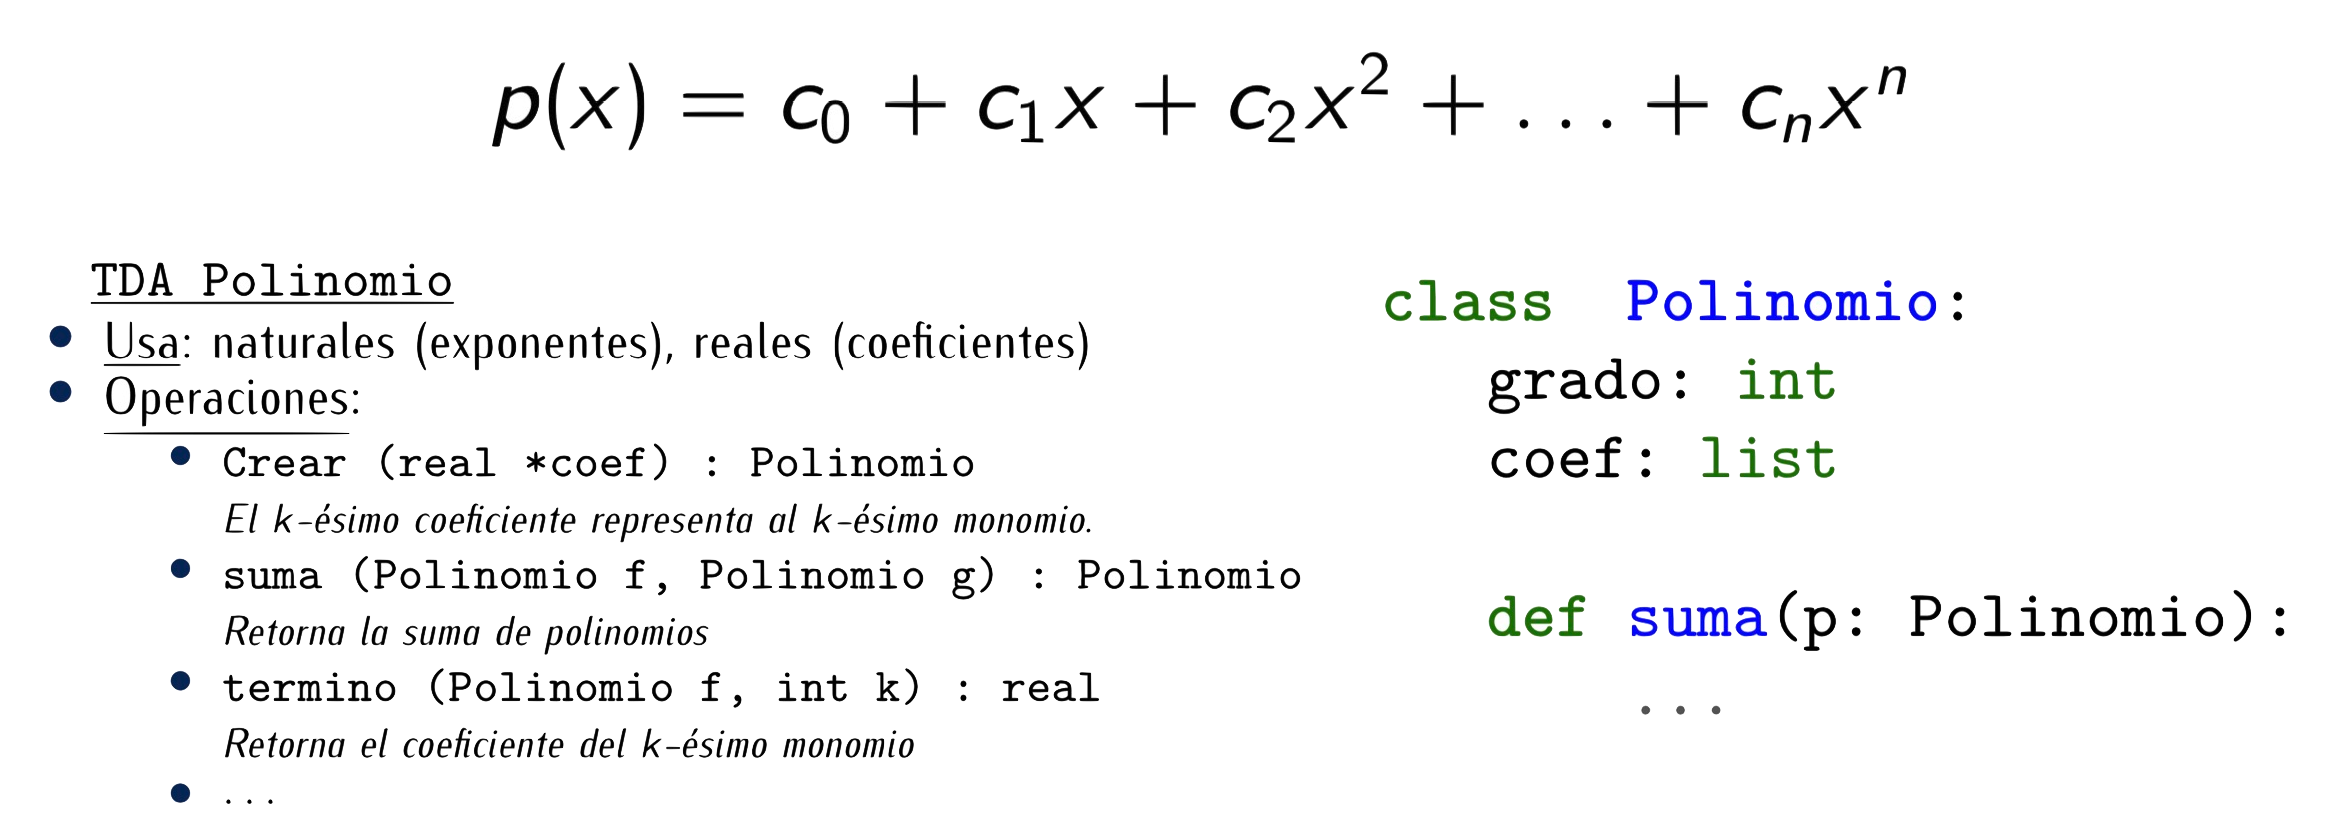
\includegraphics[width=.8\textwidth, height=.18\textheight]{fig/polinomio}
}

\graphicspath{{img/}}




%%%%%%%%%%%%%%%%%%%%%%%%%%%%%%%%%%
%%%%%%%%%%%%%%%%%%%%%%%%%%%%%%%%%%
%%%%%%%%%%%%%%%%%%%%%%%%%%%%%%%%%%
%%%%%%%%%%%%%%%%%%%%%%%%%%%%%%%%%%

%https://es.overleaf.com/learn/how-to/Writing_Markdown_in_LaTeX_Documents
\usepackage[hashEnumerators]{markdown}


%%%%%%%%%%%%%%%%%%%%%%%%%%%%%%%%%%
%%%%%%%%%%%%%%%%%%%%%%%%%%%%%%%%%%
%%%%%%%%%%%%%%%%%%%%%%%%%%%%%%%%%%
%%%%%%%%%%%%%%%%%%%%%%%%%%%%%%%%%%
\begin{document}

%\pgfdeclareimage[height=1cm]{logo}{logo.png}
%\logo{\pgfuseimage{logo}}



%--------------------------------------------------------------------------------
{\usebackgroundtemplate{%
  \includegraphics[width=\paperwidth,height=\paperheight]{../img/fondoUMUCompleto}}

\begin{frame}[b]
	\maketitle

\begin{tikzpicture}[overlay, remember picture]
\node[anchor=south west, %anchor is bottom left corner of the graphic
      xshift=.43\textwidth, %shifting around
      yshift=0.7cm] 
     at (current page.south west) %left bottom corner of the page
     {\includegraphics[width=.3\textwidth, height=.3\textheight]{fig/evolucionHumana}
     \footnote[frame]{\tiny
Imagen: Evolución Humana: \url{https://images.app.goo.gl/BisXt9wS8na9vfgP9} }}; 
\end{tikzpicture}
	
\end{frame}			% Transparencia: Título
}


%--------------------------------------------------------------------------------
%%%%%%%%%%%%%%%%%%%%%%%%%%%%%%%%%%
%%%%%%%%%%%%%%%%%%%%%%%%%%%%%%%%%%
\begin{frame}{Índice de Contenidos}\tableofcontents \end{frame}


%%%%%%%%%%%%%%%%%%%%%%%%%%%%%%%%%%%%%
%%%%%%%%%%%%%%%  SECTION   %%%%%%%%%%%%%%%
%%%%%%%%%%%%%%%%%%%%%%%%%%%%%%%%%%%%%
\section{Relaciones}



%%%%%%%%%%%%%%%%%%%%%%%%%%%%%%%%%%%%%
%%%%%%%%%%%%%%%%%%%%%%%%%%%%%%%%%%%%%
\subsection{Tipos de Relaciones} 

%%%%%%%%%%%%%%%%%%%%%%%%%%%%%%%%%%%%%
%%%%%%%%%%%%%%%%%%%%%%%%%%%%%%%%%%%%%
\begin{frame}{Relaciones entre clases}  

\begin{itemize} 
\item Cuando se tiene varios tipos de objetos,  pueden existir vínculos entre ellos. 

\item A los vínculos se llaman \key{relaciones}.

\item En su versión más sencilla  un objeto simplemente manda un mensaje a otro.

\item En su versión más compleja un objeto usa toda la información contenida en otro

\item Distinguimos los siguientes tipos de relaciones de menor a mayor dependencia:

\begin{itemize} 
\item Relación de uso
\item Asociación
\item Agregación (has-a)
\item Composición (part-of)
\item Herencia (is-a)
\end{itemize}


\item Estas relaciones establecen una relación jerárquica (no estricta) entre clases.

\item \key[blue]{Cuándo definir uno u otro tipo de relación dependerá del diseño final (interpretación del programador y principios de ingeniería informática).}

\end{itemize}


\end{frame}
% . . . . . . . . . . . . . . . . . . . . . . . . . . . . . . . . . . . . . . . . . . . . . . . . . . . . . . 
% . . . . . . . . . . . . . . . . . . . . . . . . . . . . . . . . . . . . . . . . . . . . . . . . . . . . . . 




%%%%%%%%%%%%%%%%%%%%%%%%%%%%%%%%%%%%%
%%%%%%%%%%%%%%%%%%%%%%%%%%%%%%%%%%%%%
\begin{frame}[fragile]{Relación de uso} 

\begin{itemize}
\item Una \key{relación de uso} es una relación en la que una clase utiliza objetos de otra clase, pero es una \textbf{relación esporádica}. Es la relación más general posible entre dos clases.
\end{itemize}

\begin{columns}
\begin{column}{.49\textwidth}
\begin{itemize}
\item Para indicar que una clase A usa una clase B, se representa por:
\centerline{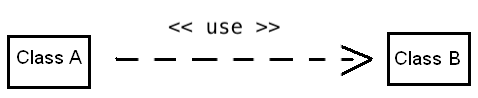
\includegraphics[width=.8\textwidth]{fig/usaUML}}

\item Lo más típico es que se pase una instancia de la clase B a un método de la clase A.

\end{itemize}

\end{column}
\begin{column}{.41\textwidth}
 \scriptsize
\begin{pyconsole}[][frame=single]
class B:
    def use(self):
        print('me utilizan')
        
class A:
    def metodo(self, b):
        b.use()
        
a = A(); b = B(); a.metodo(b)

\end{pyconsole}

\end{column}
\end{columns}

\

\begin{itemize}
\item \textbf{Ejemplos:} \it \small
\begin{itemize}
\item Las personas usan los cajeros (sin que la persona sea cliente del banco)

\item Las personas compran en (se relacionan con) los supermercados

\item Una persona puede usar un servicio público (vehículos, correos, ayudas, ...)

\item etc ...
\end{itemize}

\end{itemize}



\end{frame}
% . . . . . . . . . . . . . . . . . . . . . . . . . . . . . . . . . . . . . . . . . . . . . . . . . . . . . . 
% . . . . . . . . . . . . . . . . . . . . . . . . . . . . . . . . . . . . . . . . . . . . . . . . . . . . . . 







%%%%%%%%%%%%%%%%%%%%%%%%%%%%%%%%%%%%%
%%%%%%%%%%%%%%%%%%%%%%%%%%%%%%%%%%%%%
\begin{frame}[fragile]{Relación Asociación} 

\begin{itemize}
\item La \key{relación de asociación} es una \textbf{relación de uso} (un objeto le requiere a otro objeto que desarrolle un servicio por él - paso de mensajes), \textbf{y 
además} se quiere que sea una relación de dependencia \textbf{estable en el tiempo}.

\end{itemize}



\begin{columns}
\begin{column}{.50\textwidth}
\begin{itemize}
\item Para indicar que una clase A está asociada (depende de) una clase B, se representa por:
\centerline{\includegraphics[clip, viewport=0 250 500 400, width=.8\textwidth]{fig/asociacionUML}}

\end{itemize}

\end{column}
\begin{column}{.41\textwidth}
 \scriptsize
\begin{pyconsole}[][frame=single]
class B:
    pass
    
class A:
    def __init__(self, b):
        # A depende de B
        self.__b = b  

\end{pyconsole}

\end{column}
\end{columns}


\begin{itemize}
\item Un atributo de A es una instancia de B

\item La existencia de As no depende de la existencia de Bs (el atributo puede quedar nulo)
\end{itemize}


\

\begin{itemize}
\item \textbf{Ejemplos:} \it \small
\begin{itemize}
\item Un cliente web depende de un servidor (cambia en el tiempo)

\item Los estudiantes se relacionan con los profesores, y a la inversa (cambian en el tiempo).

\item Los propietarios de casas se relacionan con sus aseguradoras (cambian en el tiempo).

\item etc ...
\end{itemize}

\end{itemize}

\end{frame}
% . . . . . . . . . . . . . . . . . . . . . . . . . . . . . . . . . . . . . . . . . . . . . . . . . . . . . . 
% . . . . . . . . . . . . . . . . . . . . . . . . . . . . . . . . . . . . . . . . . . . . . . . . . . . . . . 



%%%%%%%%%%%%%%%%%%%%%%%%%%%%%%%%%%%%%
%%%%%%%%%%%%%%%%%%%%%%%%%%%%%%%%%%%%%
\begin{frame}[fragile]{Agregación} 

\begin{itemize}
\item Una \key{relación de agregación} es un caso particular de asociación.
\item Se produce cuando una objeto \key{tiene-un} objeto \fbox{relación 'has-a'}
\end{itemize}

\begin{columns}
\begin{column}{.49\textwidth}
\begin{itemize}

\item Para indicar que una clase A tiene-un objeto de B y/o B es parte de A se representa por:
\centerline{\includegraphics[clip, viewport=0 120 500 250, width=.8\textwidth]{fig/asociacionUML}}
\end{itemize}

\end{column}
\begin{column}{.41\textwidth}
 \scriptsize
\begin{pyconsole}[][frame=single]
class B:
    pass
    
class A:
    def __init__(self, b):
        # A depende de B
        self.__b = b  

\end{pyconsole}

\end{column}
\end{columns}

\begin{itemize}

\item Al igual que en la relación de asociación, la relación \key{no afecta a sus ciclos de vida}: aunque \key{A tiene un miembro del tipo  B}. Si destruyes A, sigue existiendo B. 
\item Los objetos pueden existir independientemente

\vskip -0.15 cm


\item \textbf{Ejemplos:} \it \small
\begin{itemize}
\item Una factura está asociado a un cliente (y el cliente puede aparecer en varias facturas)

\item Una persona puede tener un coche/jersey (y el coche/jersey puede existir sin la persona)

\item Una habitación puede tener una o varias sillas (y éstas pueden existir sin la habitación)

\item Un estudiante vive en una dirección postal (y ésta existe sin el estudiante)

\item Una biblioteca tiene estudiantes (y sin éstos, la biblioteca existe)

\item etc ...
\end{itemize}


\end{itemize}

\end{frame}
% . . . . . . . . . . . . . . . . . . . . . . . . . . . . . . . . . . . . . . . . . . . . . . . . . . . . . . 
% . . . . . . . . . . . . . . . . . . . . . . . . . . . . . . . . . . . . . . . . . . . . . . . . . . . . . . 





%%%%%%%%%%%%%%%%%%%%%%%%%%%%%%%%%%%%%
%%%%%%%%%%%%%%%%%%%%%%%%%%%%%%%%%%%%%
\begin{frame}{Composición} 

\begin{itemize}\setlength{\itemsep}{0cm}
\item La \key{relación de composición} es más restrictiva que la agregación (relación 'has-a').

\item Se produce cuando una objeto es \key{parte-de} otro objeto \fbox{relación 'part-of'}

\item Además la relación \key{sí afecta a sus ciclos de vida}: un objeto NO puede existir sin el otro.


\centerline{\includegraphics[clip, viewport=0 0 500 125, width=.4\textwidth]{fig/asociacionUML}}

\centerline{\fbox{\key{A tiene un miembro del tipo  B}. Si destruyes A, también se destruye B.}}
\centerline{\footnotesize Además: si B no está en A, el objeto A está incompleto (sin definir).}


\item \textbf{Ejemplos:} \it \small
\begin{itemize}
\item Una persona tiene corazón  (sin él la persona está incompleta)

\item Un rabo forma parte de los perros y  gatos (y sin él la mascota está incompleta)

Si dejan de existir las mascotas, dejan de existir los rabos.

\item Una biblioteca tiene libros (pero sin éstos, la biblioteca deja de existir)

\item Las habitaciones forman parte de un casa -aunque sea una.\\
Sin habitaciones no tiene sentido que eso sea una casa.\\
Si deja de existir la vivienda, deja de existir las habitaciones.

\item etc ...
\end{itemize}

\end{itemize}


\end{frame}
% . . . . . . . . . . . . . . . . . . . . . . . . . . . . . . . . . . . . . . . . . . . . . . . . . . . . . . 
% . . . . . . . . . . . . . . . . . . . . . . . . . . . . . . . . . . . . . . . . . . . . . . . . . . . . . . 





%%%%%%%%%%%%%%%%%%%%%%%%%%%%%%%%%%%%%
%%%%%%%%%%%%%%%%%%%%%%%%%%%%%%%%%%%%%
\begin{frame}[fragile]{Resumen} 

\begin{itemize}
\item A veces la diferencia entre las relaciones no está clara (depende del diseño)
\item Estarás en una situación de \key{relación de uso} cuando un objeto de B no se almacena en ningún campo de A.
\item Si el objeto se almacena en algún campo, un objeto B será un atributo del objeto A.

\begin{itemize}
	\item Si no afecta a sus ciclos de vida (destruyes A entonces el objeto B seguirá existiendo):

	\begin{itemize}
	\item Será una relación de \key{Asociación} cuando no sea de Agregación.
	\item Será una relación de \key{Agregación} cuando:\\
		$\bullet$ A tiene o posee otro objeto B,  \\
		$\bullet$  y/o B es parte de A
	\end{itemize}

\item Si sí afectan a sus ciclos de vida (destruyes A entonces el objeto B deja de existir):

	\begin{itemize}
	\item Será una relación de \key{Composición}.
	\item[-] Normalmente cuando la relación es de \textbf{agregación con aridad 1 a 1}.
	\item[-] En Java se recomienda usar la palabra \cm{final} para el atributo. Fuerza a que el objeto ``propietario'' no puede ser creado si no se inicializa con el objeto miembro (que ya debe de existir).
	\end{itemize}
\end{itemize}


\item \unEjemplo Imagina un pirata con una pata de palo, espada al cinto y disparando un cañón de su barco pirata. El pirata tiene las siguientes relaciones:
	\begin{itemize}
	\item relación de uso con el cañón (no puede llevar el cañón encima)
	\item una asociación con la espada (podría llevar encima otra arma como una pistola)
	\item una pata de palo agregada (es parte del pirata, pero sobrevive si matan al pirata)
	\item se compone de una pierna ``normal'' y brazos (son parte del pirata que no sobrevivirán si matan al pirata)
	\end{itemize}
	
\end{itemize}
\end{frame}
% . . . . . . . . . . . . . . . . . . . . . . . . . . . . . . . . . . . . . . . . . . . . . . . . . . . . . . 
% . . . . . . . . . . . . . . . . . . . . . . . . . . . . . . . . . . . . . . . . . . . . . . . . . . . . . . 


%%%%%%%%%%%%%%%%%%%%%%%%%%%%%%%%%%%%%
%%%%%%%%%%%%%%%%%%%%%%%%%%%%%%%%%%%%%
\begin{frame}{Resumen (con ejemplo)}
{Fuente: \url{http://www.cs.utsa.edu/~cs3443/uml/uml.html} }

\begin{columns}
\begin{column}{.51\textwidth}
\begin{itemize}
\item \key{Dependencia}: Persona tiene un método que usa un objeto de la clase Libro.
\item \key{Asociación}: 
\begin{itemize}
\item \key{Unidireccional}. Una persona tiene el campo \cm{owns} que almacena una lista de libros que usa. A su vez un libro lo puede usar muchas personas.
\item \key{Bidireccional}. Un libro también tiene un campo con los nombres de las personas.
\end{itemize}

\item \key{Agregación}. Se considera que el libro tiene como único propietario a una persona. De alguna forma, la persona tiene ``su ejemplar''.

\item \key{Composición}. Se considera que el libro tiene DRM  (es la única persona que puede usarlo). Si la persona muere nadie puede usarlos.
\end{itemize}
\end{column}
\begin{column}{.38\textwidth}
\centerline{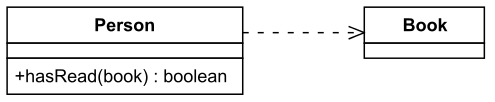
\includegraphics[width=\textwidth]{fig/dependency}}

\

\centerline{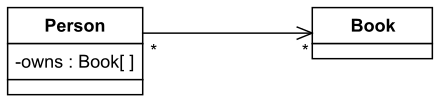
\includegraphics[width=\textwidth]{fig/unidirectional}}

\

\centerline{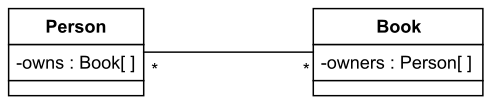
\includegraphics[width=\textwidth]{fig/bidirectional}}

\

\centerline{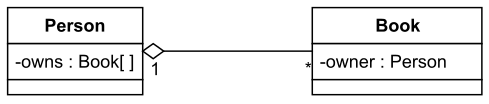
\includegraphics[width=\textwidth]{fig/aggregation}}

\

\centerline{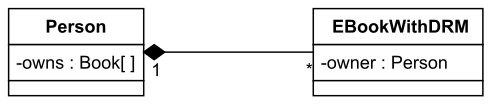
\includegraphics[width=\textwidth]{fig/composition}}

\end{column}
\end{columns}

\tiny
En \url{https://www.guru99.com/association-aggregation-composition-difference.html} tiene una lectura muy breve que compara asociación, agregación y composición.
\end{frame}
% . . . . . . . . . . . . . . . . . . . . . . . . . . . . . . . . . . . . . . . . . . . . . . . . . . . . . . 
% . . . . . . . . . . . . . . . . . . . . . . . . . . . . . . . . . . . . . . . . . . . . . . . . . . . . . . 





%%%%%%%%%%%%%%%%%%%%%%%%%%%%%%%%%%%%%
%%%%%%%%%%%%%%%%%%%%%%%%%%%%%%%%%%%%%
\begin{frame}[fragile]{Agregación vs Composición (con código)} 

\begin{itemize}
\item Observa bien las diferencias.
\item La mesa tiene dos referencias, pero cada habitación tiene solo una.
\end{itemize}

\footnotesize
\begin{pyverbatim}[][frame=single]
class Habitacion:
    ...
    def setMesa(self, mesa):
        """ 
        AGREGACIÓN. La mesa ya existe.
        Sintácticamente igual que ASOCIACIÓN.
        """
        self._mesa = mesa; 

class Casa:
    def __init__(self, numHabitaciones):
        """
        COMPOSICIÓN. Los objetos "part-of" se crean en el constructor
        """
        self.habitaciones = []     
        for i in range(0, numHabitaciones): 
            self._habitaciones.add(Habitacion()) 
            # Se crean las habitaciones
}  
\end{pyverbatim}

\end{frame}
% . . . . . . . . . . . . . . . . . . . . . . . . . . . . . . . . . . . . . . . . . . . . . . . . . . . . . . 
% . . . . . . . . . . . . . . . . . . . . . . . . . . . . . . . . . . . . . . . . . . . . . . . . . . . . . . 





%%%%%%%%%%%%%%%%%%%%%%%%%%%%%%%%%%%%%
%%%%%%%%%%%%%%%  SECTION   %%%%%%%%%%%%%%%
%%%%%%%%%%%%%%%%%%%%%%%%%%%%%%%%%%%%%
\subsection{Delegación}




%%%%%%%%%%%%%%%%%%%%%%%%%%%%%%%%%%%%%
%%%%%%%%%%%%%%%%%%%%%%%%%%%%%%%%%%%%%
\begin{frame}[fragile]{Delegación: !`Debe aplicarse siempre!} 

\begin{itemize}
\item \key{Delegación:} Cuando una clase contiene una o más instancias de otras clases, entonces la clase \textit{\bf delega} su funcionalidad a los atributos.

\item Un objeto recibe una petición y \textit{\bf delega} la ejecución del método a otros objetos.

\item Es una buena costumbre que la acción y la acción delegada tengan \textbf{el mismo nombre}.

\end{itemize}

\small
\unEjemplo La docencia en la universidad se delega a los centros, los centros a los departamentos y los departamentos a los profesores.

\scriptsize
\begin{pyverbatim}[][frame=single]
class Punto:
    def __init__(self, x: float, y: float):
       pass
    def trasladar(distancia: Punto):
       self._x += distancia.x  # Propiedades
       self._y += distancia.y
             
class Rectangulo:
    def __init__(self, largo: float, ancho: float, origen: Punto):
       self._largo = largo
       self._ancho = ancho
       self._origen = origen

   def trasladar(distancia: Punto):
      self._origen = sel._origen.trasladar(distancia) # Delegación
\end{pyverbatim}


\end{frame}
% . . . . . . . . . . . . . . . . . . . . . . . . . . . . . . . . . . . . . . . . . . . . . . . . . . . . . . 
% . . . . . . . . . . . . . . . . . . . . . . . . . . . . . . . . . . . . . . . . . . . . . . . . . . . . . . 




%%%%%%%%%%%%%%%%%%%%%%%%%%%%%%%%%%%%%
%%%%%%%%%%%%%%%  SECTION   %%%%%%%%%%%%%%%
%%%%%%%%%%%%%%%%%%%%%%%%%%%%%%%%%%%%%
\subsection{Clonación/Copia de un Objeto}




%%%%%%%%%%%%%%%%%%%%%%%%%%%%%%%%%%%%%
%%%%%%%%%%%%%%%%%%%%%%%%%%%%%%%%%%%%%
\begin{frame}{?`Cómo clonar un objeto?} 

\begin{columns}
\begin{column}{.6\textwidth}
\begin{itemize}
\item Cuando se tienen dos objetos, \cm{obj1} y \cm{obj2}, la asignación \cm{obj1=obj2} produce aliasing sobre el mismo objeto. En ningún caso hace una copia del objeto.

\item Hacer una copia conlleva mantener las relaciones de asociación, agregación y composición que tiene el objeto original, si las hubiera.

La tarea no siempre es trivial.

\item \key{Copia Superficial}

\begin{itemize}
\item Generar una instancia de la misma clase y copiar los valores de los atributos.
\item !`!` Puede existir aliasing en los atributos !!
\end{itemize}

\item \key{Copia Profunda}


\begin{itemize}
\item Además de la copia superficial realiza una copia de todos los objetos a los que se refiera.
\item Puede llegar a ser muy compleja.
\end{itemize}


\end{itemize}

\end{column}


\begin{column}{.3\textwidth}

\centerline{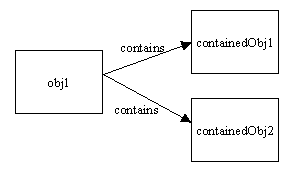
\includegraphics[height=.2\textheight]{fig/obj1}}

\centerline{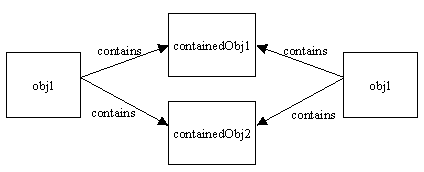
\includegraphics[height=.2\textheight]{fig/copia1}}

\

\centerline{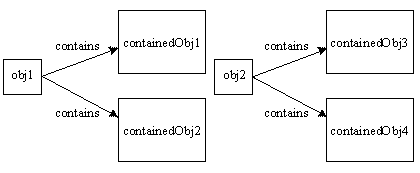
\includegraphics[height=.2\textheight]{fig/copia2}}

\end{column}
\end{columns}

\begin{itemize}
\item 
 Existen \key{otras formas} de copiar objetos:
\begin{itemize}
\item \href{http://www.javapractices.com/topic/TopicAction.do?Id=15}{Defensive copying},
\href{http://www.javapractices.com/topic/TopicAction.do?Id=12}{Copy constructors},
\href{http://www.javapractices.com/topic/TopicAction.do?Id=21}{Factory methods}.
\end{itemize}
\end{itemize}


\end{frame}
% . . . . . . . . . . . . . . . . . . . . . . . . . . . . . . . . . . . . . . . . . . . . . . . . . . . . . . 
% . . . . . . . . . . . . . . . . . . . . . . . . . . . . . . . . . . . . . . . . . . . . . . . . . . . . . . 




%%%%%%%%%%%%%%%%%%%%%%%%%%%%%%%%%%%%%
%%%%%%%%%%%%%%%%%%%%%%%%%%%%%%%%%%%%%
\begin{frame}[fragile]{Clonación de objetos en \cm[red]{Python}} 

\begin{itemize}
\item El módulo \cm{copy} permite hacer copias. 
\item Usa las funciones del módulo \cm{pickle} para la (de-)serilización de objetos.
\item Tiene los siguientes métodos:

\begin{itemize}
\item \cm{copy.copy(x)} para realizar una copia superficial de \cm{x}.
\item \cm{copy.deepcopy(x[,memo])} para realizar una copia profunda de \cm{x}.

Para evitar la copia recursiva o la copia de demasiados objetos
\begin{itemize}
\item Mantiene un diccionario \cm{memo} de los objetos ya copiados.
\item Permite al usuario redefinir los operadores de copia.
\end{itemize}
\end{itemize}

\item Para que una clase defina su propia implementación de \cm{copy}, puede definir métodos especiales \cm{\_\_copy\_\_()} y \cm{\_\_deepcopy\_\_()}.

{\small Detalles para la implementación profunda ver \scriptsize \url{https://docs.python.org/3/library/copy.html}}

\item Hay funciones que realizan copias:
\begin{itemize}
\item \cm{list()} crea una lista nueva a partir de su argumento (si puede)
\item \cm{dict.copy()} crea una copia superficial del diccionario \cm{dict}
\end{itemize}

\end{itemize}

\end{frame}
% . . . . . . . . . . . . . . . . . . . . . . . . . . . . . . . . . . . . . . . . . . . . . . . . . . . . . . 
% . . . . . . . . . . . . . . . . . . . . . . . . . . . . . . . . . . . . . . . . . . . . . . . . . . . . . . 










%%%%%%%%%%%%%%%%%%%%%%%%%%%%%%%%%%%%%
%%%%%%%%%%%%%%%%%%%%%%%%%%%%%%%%%%%%%
\begin{frame}[allowframebreaks]{Ejercicios - }



\begin{ejercicio}{}
Realiza el diagrama completo de las siguientes relaciones que existe entre estas clases, indicando si es asociación, has-a o part-of:

\hfil \begin{minipage}{.6\textwidth}
\begin{itemize}
\item Una universidad y los departamentos.
\item Un departamento y los profesores.
\item Los profesores y los alumnos.
\item Los alumnos y un grado.
\item Un grado y las asignaturas del grado.
\item Las asignaturas y los profesores.
\end{itemize}
\end{minipage}

\end{ejercicio}


\begin{ejercicio}{}
Modela la siguiente situación. Todos los piratas tienen corazón pero su número de piernas puede ir de 0 a 2. Además alguna pierna puede ser una pata de palo.

Explica el tipo de asociación y como se pondría de relieve con el correspondiente código.
\end{ejercicio}


\begin{ejercicio}{}
Representa y codifica las siguientes relaciones:

\hfil \begin{minipage}{.6\textwidth}
\begin{itemize}
\item Un usuario saca dinero de un cajero con una tarjeta, si es válida.
\item Las personas se añaden a una familia y la familia se actualiza con las personas. Una familia se entiende como una lista de personas.
\item Polígono cerrado en el plano, entendiendo como tal a una lista de puntos.
\end{itemize}
\end{minipage}
\end{ejercicio}




\begin{ejercicio}{}
Si el estado de una pareja queda determinado únicamente por su nombre y su pareja, 

\hfil \begin{minipage}{.6\textwidth}
\begin{itemize}
\item ?`cómo se construye que una persona A es soltera? 
\item ?`y si tiene pareja? Si A es pareja de B, ?`cómo se pueden construir A y B?
\item Indica el tipo de variables que intervienen en todo el proceso.
\end{itemize}
\end{minipage}

%\item Construye el psudocódigo para construir una biblioteca supuesto que tienes un constructor de libros que construye libros al azar.
\end{ejercicio}





\begin{ejercicio}{}
Un usuario sabe que está inscrito en una biblioteca y en una tienda de libros.
Tanto la biblioteca como la tienda contienen una cantidad ingente de libros tienen registrado al usuario como cliente. Además todo libro agrega la biblioteca en la que se encuentra depositado y la tienda en la que fue comprado. ¿Qué debería de hacer el usuario para consultar la disponibilidad de un libro?
\end{ejercicio}


\begin{ejercicio}{}
En un videojuego de acción en tercera persona  los jugadores controlan a un personaje. El personaje tiene la capacidad de disparar; es decir puede realizar ciertas acciones entre las que se encuentra la de  transportar un arma que puede ser disparada.
También tiene la capacidad de recoger objetos del entorno del juego; es decir puede interactuar con los objetos y en particular tiene un inventario en el que se pueden añadir objetos. ¿Cuáles son las clases y métodos que permiten similar las acciones de disparar y recoger objetos?
\end{ejercicio}



\end{frame}
% . . . . . . . . . . . . . . . . . . . . . . . . . . . . . . . . . . . . . . . . . . . . . . . . . . . . . . 
% . . . . . . . . . . . . . . . . . . . . . . . . . . . . . . . . . . . . . . . . . . . . . . . . . . . . . . 




%%%%%%%%%%%%%%%%%%%%%%%%%%%%%%%%%%%%%
%%%%%%%%%%%%%%%  SECTION   %%%%%%%%%%%%%%%
%%%%%%%%%%%%%%%%%%%%%%%%%%%%%%%%%%%%%
\section{Herencia}

%%%%%%%%%%%%%%%%%%%%%%%%%%%%%%%%%%%%%
%%%%%%%%%%%%%%%  SECTION   %%%%%%%%%%%%%%%
%%%%%%%%%%%%%%%%%%%%%%%%%%%%%%%%%%%%%
\subsection{Concepto y Tipos}


%%%%%%%%%%%%%%%%%%%%%%%%%%%%%%%%%%%%%
%%%%%%%%%%%%%%%%%%%%%%%%%%%%%%%%%%%%%
\begin{frame}{Introducción a la Herencia} \large

\begin{itemize}
\item Las \key[red]{clases de objetos} pueden verse como \key{conjunto de elementos}, cada uno caracterizado por su estado y su comportamiento.

\item Como conjuntos, sus elementos pueden compartirse o no.

\item Matemáticamente, si se comparte se habla de \key{intersección}.

\begin{itemize} \normalsize
\item La intersección de dos conjuntos es el conjunto formado por los elementos comunes.
\end{itemize}

\item Cuando la intersección entre dos conjuntos es no vacía entonces puede ocurrir
\begin{itemize} \normalsize
\item Solo se comparten algunos elementos.
\item Un conjunto comparte todos los elementos con otro. \\
	En este caso se dice que el primero está incluido en el segundo.
\end{itemize}

\item Este tema va de \key{inclusiones de clases}.

\item En POO a la inclusión se le llama \key{herencia}.
\end{itemize}
\end{frame}
% . . . . . . . . . . . . . . . . . . . . . . . . . . . . . . . . . . . . . . . . . . . . . . . . . . . . . . 
% . . . . . . . . . . . . . . . . . . . . . . . . . . . . . . . . . . . . . . . . . . . . . . . . . . . . . . 



%%%%%%%%%%%%%%%%%%%%%%%%%%%%%%%%%%%%%
%%%%%%%%%%%%%%%%%%%%%%%%%%%%%%%%%%%%%
\begin{frame}{Herencia} 

\begin{itemize}

\item Ya sabe que las clases se pueden relacionar entre ellas por asociación. En particular 

\begin{itemize}
\item La asociación de  \key{agregación} se corresponde con las relación \key{\tt has-a}
\item La asociación de \key{composición} se corresponde con las relación  \key{\tt part-of}.
\end{itemize}

\item La asociación entre clases de \key{herencia} se corresponde con la relación \key{\tt  Is-a}

\item Se usa cuando una clase es una \key{generalización} de otra o, si se prefiere, cuando la otra es \key{un caso particular} de la una.
\end{itemize}

\unEjemplo 

\centerline{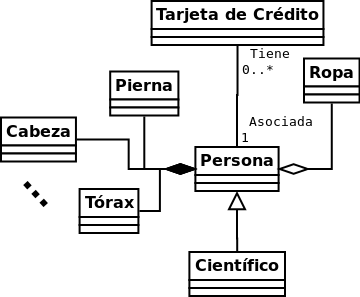
\includegraphics[width=.4\textwidth]{fig/relaciones}}


\centerline{\scriptsize Fuente: \url{http://fundamentospoorrr.blogspot.com/2019/03/composicion-agregacion-y-asociacion.html}}
\end{frame}
% . . . . . . . . . . . . . . . . . . . . . . . . . . . . . . . . . . . . . . . . . . . . . . . . . . . . . . 
% . . . . . . . . . . . . . . . . . . . . . . . . . . . . . . . . . . . . . . . . . . . . . . . . . . . . . . 




%%%%%%%%%%%%%%%%%%%%%%%%%%%%%%%%%%%%%
%%%%%%%%%%%%%%%%%%%%%%%%%%%%%%%%%%%%%
\begin{frame}{Subclases} 

\begin{itemize}
\item La herencia crea \key{clases nuevas a partir de una clase existente}.
\begin{itemize}
\item La clase nueva \key[red]{es un} caso particular de la clase que ya existe.
\end{itemize}

\item A la clase nueva se le denomina \key{subclase}  y a la existente \key{superclase} 
\begin{itemize}
\item Responden a una \key{especialización} y a una \key{generalización}, respectivamente.
\end{itemize}
	
\item \key{Nombres alternativos }
\begin{itemize}
\item Para la \textbf{subclase}: clase hija, derivadas o subtipos. 
\item Para la \textbf{superclase}: clase padre o base.
\end{itemize}

\item La herencia es el proceso por el que una \key{clase hija reconoce a los miembros de la clase padre}.
\begin{itemize}
\item Los miembros reconocidos se llaman \key{miembros heredados}
\item En principio, no tiene que reconocer a todos (\key{sólo los que se indiquen}).
\end{itemize}

\item En la subclase \key{se DEBEN definir nuevos miembros} (atributos y/o  métodos)
\begin{itemize}
\item Por eso se dice que la clase derivada \key{extiende} a la clase base.
\item Los nuevos miembros  serán \key{desconocidos} por la clase padre.
\end{itemize}

\end{itemize}
\end{frame}
% . . . . . . . . . . . . . . . . . . . . . . . . . . . . . . . . . . . . . . . . . . . . . . . . . . . . . . 
% . . . . . . . . . . . . . . . . . . . . . . . . . . . . . . . . . . . . . . . . . . . . . . . . . . . . . . 





%%%%%%%%%%%%%%%%%%%%%%%%%%%%%%%%%%%%%
%%%%%%%%%%%%%%%%%%%%%%%%%%%%%%%%%%%%%
\begin{frame}{Tipos de Herencia}
\begin{itemize} 
\item Hay \key{herencia simple} cuando la subclase solo puede heredar de una clase padre. 

Visualmente, el gráfico UML tiene forma de árbol.

\centerline{\includegraphics[width=.4\textwidth]{fig/poo-images-animaux}}

\item Hay \key{herencia múltiple} cuando la subclase hereda de dos o más padres.

Visualmente, el gráfico tiene forma de grafo.
\end{itemize}

\centerline{\includegraphics[width=.4\textwidth]{fig/poo-images-animaux2}}



\begin{itemize}
\item \small Un objeto con ``tipo de dato'' de una subclase también es un ``tipo de dato'' de una superclase de la misma rama.
\small P.e. un objeto de tipo hombre también es de tipo omnívoro y animal.
\end{itemize}

\vfill

\centerline{\scriptsize Fuente: \url{https://es.ccm.net/contents/411-poo-herencia}}
\end{frame}
% . . . . . . . . . . . . . . . . . . . . . . . . . . . . . . . . . . . . . . . . . . . . . . . . . . . . . . 
% . . . . . . . . . . . . . . . . . . . . . . . . . . . . . . . . . . . . . . . . . . . . . . . . . . . . . . 





%%%%%%%%%%%%%%%%%%%%%%%%%%%%%%%%%%%%%
%%%%%%%%%%%%%%%%%%%%%%%%%%%%%%%%%%%%%
\begin{frame}{Herencia en \cm[red]{Java}} 

\begin{itemize}
\item En Java \key{la herencia es simple} y no admite herencia múltiple.

\item El modificador \cm{protected} es un modificador específico para la herencia de miembros.

\item Con éste, ya tenemos todos los modificadores de visualización de Java:

\centerline{\scriptsize\begin{tabular}{|c||c|c|c|c|} \hline
\textbf{Modificador} & \textbf{Clase} & \textbf{Package} & \textbf{Subclase} & \textbf{Todos} \\ \hline \hline
\textbf{public} & Sí & Sí  & Sí  & Sí \\
\textbf{protected} & Sí & Sí  & Sí  & \key[red]{No} \\
\textbf{No especificado} (friendly) & Sí & Sí  & \key[red]{No}  & \key[red]{No} \\
\textbf{private} & Sí & \key[red]{No}  & \key[red]{No}  & \key[red]{No} \\ \hline
\end{tabular}}

\item Definición de subclases: \cm[blue]{class} \cm{Subclase} \underline{\cm[blue]{extends} \cm{Superclase}} {\tt \{...\}}

\item \cm[blue]{extends}  se usa para generar una subclase (especialización) de un tipo de objeto.

\item Una subclase puede (debe) llamar al constructor del padre con \cm{super()}.

\end{itemize}

\vskip -.25cm 

\begin{columns}
\begin{column}{.65\textwidth}


\begin{itemize}
\item \cm{super()} representa al constructor de la clase padre, y se llamará con tantos argumentos como requiera dicho constructor.

\item \cm{super()} debe ser siempre la primera línea de un constructor (y excluye a \cm{this()}  - uno u otro)
\end{itemize}

\end{column}
\begin{column}{.2\textwidth}
\vskip 0.1cm
\centerline{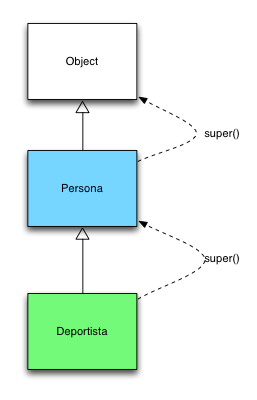
\includegraphics[width=1.5\textwidth, height=0.3\textheight]{fig/super}}
\end{column}
\end{columns}

\end{frame}
% . . . . . . . . . . . . . . . . . . . . . . . . . . . . . . . . . . . . . . . . . . . . . . . . . . . . . . 
% . . . . . . . . . . . . . . . . . . . . . . . . . . . . . . . . . . . . . . . . . . . . . . . . . . . . . . 

%
%
%%%%%%%%%%%%%%%%%%%%%%%%%%%%%%%%%%%%%%
%%%%%%%%%%%%%%%%%%%%%%%%%%%%%%%%%%%%%%
%\begin{frame}[fragile]{Ejemplo}
%
%\begin{code}
%public class Mascota {        // Una clase
%    protected String nombre;  // Miembro que heredarán las subclases
%    public Mascota(String nombre) {this.nombre = nombre;}
%    public String getNombre() {return nombre;}
%} // Fin de class
%\end{code}
%
%\vskip -0.25cm
%
%
%\begin{code}
%public class Perro extends Mascota { // Subclase
%    private String raza;             // Con miembro propio
%    public Perro(String nombre, String raza) { // Constructor
%        super(nombre);               // Invoca al constructor del padre
%        this.raza = raza; }          // Termina la definición
%    public String getRaza() {return raza;}
%} // Fin de class
%\end{code}
%
%\vskip -0.25cm
%
%
%\begin{code}
%public class Herencia {
%    public static void main(String[] args) {
%        Perro perro = new Perro("Toby", "Mastín");
%        System.out.println(perro.getNombre()+", "+perro.getRaza());
%     }
%}
%\end{code}
%
%\begin{out}
%Toby, Mastín
%\end{out}
%\end{frame}
%% . . . . . . . . . . . . . . . . . . . . . . . . . . . . . . . . . . . . . . . . . . . . . . . . . . . . . . 
%% . . . . . . . . . . . . . . . . . . . . . . . . . . . . . . . . . . . . . . . . . . . . . . . . . . . . . . 





%%%%%%%%%%%%%%%%%%%%%%%%%%%%%%%%%%%%%
%%%%%%%%%%%%%%%%%%%%%%%%%%%%%%%%%%%%%
\begin{frame}{Herencia en \cm[red]{Python}} 

\begin{itemize}
\item En Python \key{la herencia es múltiple}.

\item Se heredan todos los miembros (no existen modificadores específicos para herencia)

\item Definición de subclases: \\
\centerline{\cm[blue]{class} \cm{Subclase} \cm{\underline{(Superclase1, SuperClase2, ...)}}}

\item En herencia múltiple surge \key{el problema de la estructura del diamante}: Si \cm[blue]{B1} y \cm[blue]{B2} heradan y sobreescriben un método de \cm[blue]{A} y la clase \cm[blue]{C} no lo sobreescribe pero hereda de \cm[blue]{B1} y de \cm[blue]{B2}, entonces el método heredado en \cm[blue]{C} ...\\
\centerline{... ?`hay herencia repetida? ?`es de \cm[blue]{B1} o es de \cm[blue]{B2}? Siempre usa la primera superclase}

\item  \cm[red]{Python} usa el \key{Method Resolution Order} (MRO): crea una lista de clases que se buscan de izquierda a derecha y de abajo a arriba (\cm[blue]{C}, \cm[blue]{B1}, \cm[blue]{A}, \cm[blue]{B2}, \cm[blue]{A}) y luego elimina todas las apariciones de una clase repetida menos la última. 
\begin{itemize}
\item Por tanto, el orden de resolución del método es: (\cm[blue]{C}, \cm[blue]{B1}, \cm[blue]{B2}, \cm[blue]{A}) . \item La clase raíz siempre es \cm{object}.
\end{itemize}


\item El árbol de ancestros puede obtenerse con el atributo \cm[blue]{\_\_mro\_\_}.

\item Una subclase puede (debe) llamar al \cm[blue]{\_\_init\_\_()} del padre con \cm{super()}.

\begin{itemize}
\item \cm{super()} es una referencia indirecta calculada.
\item Retorna un \key{objeto proxy}: un objeto que delega las llamadas a los métodos correctos sin crear un objeto adicional.
\item El cálculo depende tanto de la clase desde donde \cm{super()} es llamada como del árbol de ancestros de la instancia. 
\end{itemize}

\end{itemize}

\end{frame}
% . . . . . . . . . . . . . . . . . . . . . . . . . . . . . . . . . . . . . . . . . . . . . . . . . . . . . . 
% . . . . . . . . . . . . . . . . . . . . . . . . . . . . . . . . . . . . . . . . . . . . . . . . . . . . . . 







%%%%%%%%%%%%%%%%%%%%%%%%%%%%%%%%%%%%%
%%%%%%%%%%%%%%%  SECTION   %%%%%%%%%%%%%%%
%%%%%%%%%%%%%%%%%%%%%%%%%%%%%%%%%%%%%
\subsection{Sobreescritura y Ocultación}


%%%%%%%%%%%%%%%%%%%%%%%%%%%%%%%%%%%%%
%%%%%%%%%%%%%%%%%%%%%%%%%%%%%%%%%%%%%
\begin{frame}{Sobreescritura y Ocultación} 

\begin{itemize}
\item En una superclase  se indicará siempre \key{qué miembros serán heredados}.
\begin{itemize}
\item En \cm[red]{Python}, se heredan todos.
\end{itemize}

\item Si una subclase \key{hereda un método} puede hacer dos cosas
\begin{itemize}
\item \key{Usar} el método de la superclase como si fuera suyo
\item \key{Sobreescribir} (\textit{Overriding}) el método para que el comportamiento sea diferente

La \key[red]{sobreescritura} de un método es construir un nuevo método con la misma declaración (signatura) pero donde cambia la definición.
\end{itemize}

\item Si una subclase \key{hereda una variable} puede hacer dos cosas
\begin{itemize}
\item \key{Usar} la variable de la superclase como si fuera suyo
\item \key{Ocultar} la variable heredada

La \key[red]{ocultación} de una variable es definir una variable con el mismo identificador de la variable de la superclase.

\begin{itemize}
\item \textbf{Dependiendo del lenguaje de programación:} para que realmente haya ocultación también debe coincidir el tipo de dato.
\end{itemize} 
\end{itemize}

\item \key{Cuando se sobrescriben/ocultan miembros} (métodos/variables) en una subclase, el comportamiento no es exactamente el mismo en distintos lenguajes de programación
\end{itemize}
\end{frame}
% . . . . . . . . . . . . . . . . . . . . . . . . . . . . . . . . . . . . . . . . . . . . . . . . . . . . . . 
% . . . . . . . . . . . . . . . . . . . . . . . . . . . . . . . . . . . . . . . . . . . . . . . . . . . . . . 



%%%%%%%%%%%%%%%%%%%%%%%%%%%%%%%%%%%%%
%%%%%%%%%%%%%%%%%%%%%%%%%%%%%%%%%%%%%
\begin{frame}{Sobreescritura y Ocultación en \cm[red]{Java} y \cm[red]{Python}} 

\begin{itemize}
\item \key{Cuando se sobrescriben/ocultan miembros} (métodos/variables) en una subclase, el comportamiento no es exactamente el mismo en distintos lenguajes de programación

\item \cm[red]{Java}
\begin{itemize}
\item \key{No significa que se destruyan} los miembros en la superclase.
\item Los miembros sobreescritos de la superclase  \key{estarán ocultos}.
\item Cuando en la subclase se haga \key{referencia  a los miembros sobreescritos} \textbf{siempre se hará referencia a las nuevas definiciones}.
\item Para poder \textbf{acceder a los miembros de la superclase} se deberá  usar el objeto \cm{super}.
\end{itemize}

\item \cm[red]{Python}
\begin{itemize}
\item En cuanto a los \key{métodos sobreescritos}, se comporta igual que \cm[red]{Java}: cada método tiene su propia referencia.
\item Pero este lenguaje destaca por su no-privacidad, lo que se traduce principalmente en las variables.
\item \key{Una variable}-miembro \key{estará compartida por todas las clases}: cada uno \textbf{no tendrá} la suya (a diferencia de Java). \concepto{No hay ocultación}.

%Lo que realmente pasa es que cuando se crea un objeto de la subclase, éste será asignado a self. Solo cuando se haga una  asignación se creará la referencia al atributo. Por lo que este atributo ya no cambiará

\item Para simular la ocultación, debe usarse \cm[red]{\_\_} al inicio de la variable.

Aunque internamente no dejará de ser una variable pública solo que empezará por el nombre de la clase

\item Para poder \textbf{acceder a los miembros de la superclase} se deberá  usar la función \cm{super()}.
\end{itemize}

\end{itemize}
\end{frame}
% . . . . . . . . . . . . . . . . . . . . . . . . . . . . . . . . . . . . . . . . . . . . . . . . . . . . . . 
% . . . . . . . . . . . . . . . . . . . . . . . . . . . . . . . . . . . . . . . . . . . . . . . . . . . . . . 




%%%%%%%%%%%%%%%%%%%%%%%%%%%%%%%%%%%%%
%%%%%%%%%%%%%%%%%%%%%%%%%%%%%%%%%%%%%
\begin{frame}[fragile]{Ejemplo - I}{\tacha{La subclase reconoce a los atributos de la superclase.} La superclase añade atributos a objetos de la subclase.}
\small
\begin{itemize} \setlength\itemsep{-0.2em} \small
\item \pyv{__dict__} es diccionario que muestra algunos atributos propios de un objeto.
\item \pyv{dir(obj)} es una estructura-lista que muestra sus atributos y recursivamente las heredadas por los ancestros. Muestra \pyv{__dict__} y más atributos.
\end{itemize}

\scriptsize
\begin{minipage}{.47\textwidth}
\begin{pyconsole}[][frame=single]
class Mascota: # Una clase
    def __init__(self, nombre):
        self._nombre = nombre
    def get_nombre(self):
        return self._nombre

\end{pyconsole}
\end{minipage}
\hfill
\begin{minipage}{.47\textwidth}

\begin{pyconsole}[][frame=single]
class Perro(Mascota): # Subclase
    cardinal: int = 0

perro = Perro("Toby")
print (perro.get_nombre())  
   
\end{pyconsole}
\end{minipage}

\vskip -0.25cm



\begin{pyconsole}[][frame=single]
# Atributos únicos de las clases (1) Mascota, (2) Perro y (3) el objeto perro
print([ m for m in Mascota.__dict__ if not m.startswith('__')],
      [ m for m in Perro.__dict__ if not m.startswith('__')],  perro.__dict__) 
#
# Atributos reconocidos en las clases (1) Mascota, (2) Perro y (3) el objeto perro
print([ m for m in dir(Mascota) if not m.startswith('__')],
      [ m for m in dir(Perro) if not m.startswith('__')], 
      [ m for m in dir(perro) if not m.startswith('__')])
\end{pyconsole}

\begin{itemize}\setlength\itemsep{-0.2em} \small
\item \cm[blue]{Perro} no tiene constructor, así que usa \cm{\_\_init\_\_()} de \cm[blue]{Mascota}.
\item En \cm[blue]{Mascota} se asigna el valor \cm[red]{"Toby"} a \cm{self.}{\tt\_nombre} % con \cm{self:\_\_main\_\_.Perro object at 0x11012...}.
\item Con \cm[blue]{get\_nombre()} se muestra el valor de \cm{self.}{\tt \_nombre} % con \cm{self:\_\_main\_\_.Perro object at 0x11012...}.
\item Es decir, \cm{self.}{\tt \_nombre} no cambia su referencia una vez creado el atributo.
\end{itemize}


\end{frame}
% . . . . . . . . . . . . . . . . . . . . . . . . . . . . . . . . . . . . . . . . . . . . . . . . . . . . . . 
% . . . . . . . . . . . . . . . . . . . . . . . . . . . . . . . . . . . . . . . . . . . . . . . . . . . . . . 






%%%%%%%%%%%%%%%%%%%%%%%%%%%%%%%%%%%%%
%%%%%%%%%%%%%%%%%%%%%%%%%%%%%%%%%%%%%
\begin{frame}[fragile]{Ejemplo - II}{Un ejemplo más claro donde los atributos se añaden al objeto}
\scriptsize
\begin{minipage}{.49\textwidth}
El atributo \cm{self.\_nombre} es compartido en las dos subclases.
Pero cada uno tiene su propio identificador.

\begin{pyconsole}[][frame=single]
class Mascota: # Una clase
    def __init__(self, nombre):
        self._nombre = nombre
    def get_nombre(self):
        return self._nombre
        
class Perro(Mascota): # Subclase
    def __init__(self, nombre):
    #Añade atributo nombre a self
        super().__init__(nombre)
    #Modifica el atributo nombre de self
        self._nombre = "EL " + nombre

perro = Perro("Toby")
print (perro.get_nombre())

\end{pyconsole}
\end{minipage}
\hfill
\begin{minipage}{.49\textwidth}
El atributo \cm{\_\_nombre} queda ``oculto''.\\
Realmente hay un \cm{\_\_nombre} en cada clase.
\begin{pyconsole}[][frame=single]
class Mascota: # Una clase
    def __init__(self, nombre):
        # Realmente es _Mascota__nombre
        self.__nombre = nombre
    def get_nombre(self):
        return self.__nombre
        
class Perro(Mascota): # Subclase
    def __init__(self, nombre):
        super().__init__(nombre)
        # Realmente es _Perro__nombre
        self.__nombre = "EL " + nombre
    def get_nombre(self):
        return self.__nombre

perro = Perro("Toby")
print (perro.get_nombre())
#
# Esto no está bien, pero demuestra que 
# los atributos son siempre públicos.
print (perro._Mascota__nombre)  
   
\end{pyconsole}
\end{minipage}

\end{frame}
% . . . . . . . . . . . . . . . . . . . . . . . . . . . . . . . . . . . . . . . . . . . . . . . . . . . . . . 
% . . . . . . . . . . . . . . . . . . . . . . . . . . . . . . . . . . . . . . . . . . . . . . . . . . . . . . 




%%%%%%%%%%%%%%%%%%%%%%%%%%%%%%%%%%%%%
%%%%%%%%%%%%%%%%%%%%%%%%%%%%%%%%%%%%%
\begin{frame}[fragile]{Sobreescritura  sobre la clase \cm{object}}

\begin{itemize}
\item En Python hay una clase raíz: \cm{object}
\item Algunos atributos \cm[red]{Python}  conviene sobreecribirlos. % son los siguientes. % (use \cm{dir(object)}):

\item \pyv{__init__()}. El método de inicialización de variables de un objeto.

\begin{itemize}
\item Este método siempre se tienen que sobreescribir y debe de usar \pyv{super()} - salvo que sea descendiente de \pyv{object}.
\end{itemize}


\item \pyv{__str__(self)}. El modo en el que un usuario vería la información de la clase. Retorna una cadena ``informal''.

\item \pyv{__repr__(self)}. El modo en el que un programador vería la información de la clase. Retorna una cadena ``formal''.

\item \pyv{__gt__()}, \pyv{__ge__()}, \pyv{__lt__()}, \pyv{__le__()}: Métodos que define las desigualdades lógicas al comparar dos objetos con los operadores \cm{$>$}, \cm{$>=$}, \cm{$<$} y $\cm{<=}$.

\item \pyv{__eq__(self, objeto)}. Método que define el operador de igualdad (==)

\begin{itemize}
\item Si \cm{a == b} entonces \cm{hash(a) == hash(b)}
\item Si \cm{hash(a) == hash(b)}, entonces \cm{a} puede ser igual a \cm{b}
\item Si \cm{hash(a) != hash(b)}, entonces \cm{a != b}
\item Por tanto, se debe sobreescribir \cm{\_\_hash\_\_(self, objeto)}, que es el invocado por \cm{hash()}, para que se cumplan las condiciones indicadas.
	\begin{itemize}
	\item {\scriptsize \url{https://docs.python.org/3.5/reference/datamodel.html#object.__hash__}} indica cómo
	\end{itemize}
\end{itemize}

%{\tiny
%\begin{pyverbatim}[][frame=single]
%class A:
%    def __key(self):
%        return (self.attr_a, self.attr_b, self.attr_c)
%
%    def __hash__(self):
%        return hash(self.__key())
%
%    def __eq__(self, other):
%        if isinstance(other, A):
%            return self.__key() == other.__key()
%        return NotImplemented
%\end{pyverbatim}
%}

\end{itemize}

\end{frame}
% . . . . . . . . . . . . . . . . . . . . . . . . . . . . . . . . . . . . . . . . . . . . . . . . . . . . . . 
% . . . . . . . . . . . . . . . . . . . . . . . . . . . . . . . . . . . . . . . . . . . . . . . . . . . . . . 







%%%%%%%%%%%%%%%%%%%%%%%%%%%%%%%%%%%%%
%%%%%%%%%%%%%%%  SECTION   %%%%%%%%%%%%%%%
%%%%%%%%%%%%%%%%%%%%%%%%%%%%%%%%%%%%%
\subsubsection{Problema del diamante}



%%%%%%%%%%%%%%%%%%%%%%%%%%%%%%%%%%%%%
%%%%%%%%%%%%%%%%%%%%%%%%%%%%%%%%%%%%%
\begin{frame}

\hfil\hfil\begin{minipage}{.4\textwidth}
\begin{alertblock}{Sobreescritura}
\centerline{Problema del diamante}
\end{alertblock}
\end{minipage}
\end{frame}

%%%%%%%%%%%%%%%%%%%%%%%%%%%%%%%%%%%%%
%%%%%%%%%%%%%%%%%%%%%%%%%%%%%%%%%%%%%
\begin{frame}[fragile, label=ProblemaDiamante]{Problema del Diamante}
{ Method Resolution Order(MRO)}
\scriptsize
\begin{minipage}{.48\textwidth}
Es lo que ocurre cuando una ancestro puede ser invocado dos veces por herencia.
\hfill \cm[red]{Python} lo resuelve con \cm{super()} \\
Se sigue el árbol de ancestros  definido por \cm{\_\_mro\_\_}
\begin{pyconsole}[][frame=single]
class A:
    def __init__(self):
        print("A")

class B1(A):
    def __init__(self):
        print("B1")
        super().__init__()

class B2(A):
    def __init__(self):
        print("B2")
        super().__init__()

class C(B1, B2):
    def __init__(self):
        print("C")
        super().__init__()

c = C()
 
\end{pyconsole}
\end{minipage}
\hfill
\begin{minipage}{.48\textwidth}
Si el método no está por la rama por defecto pasa a la siguiente.
\begin{pyconsole}[][frame=single]
class A:
    def __init__(self):
        print("A")

class B1(A):
    None

class B2(A):
    def __init__(self):
        print("B2")
        super().__init__()

class C(B1, B2):
    def __init__(self):
        print("C")
        super().__init__()

c = C()
\end{pyconsole}

$\bullet$ ?`Qué pasaría si \cm[blue]{B2} tampoco tuviera \cm[blue]{\_\_init\_\_()}?\\
R1: Invocaría a la clase \cm[blue]{A} que es la siguiente de la lista. \\
$\bullet$ ?`Se puede usar un método de \cm[blue]{A} sin pasar por las \cm[blue]{Bx}?\\
R: Sí, usando  \cm{super(A, self)}\cm[blue]{.metodo()}.
\end{minipage}

\end{frame}
% . . . . . . . . . . . . . . . . . . . . . . . . . . . . . . . . . . . . . . . . . . . . . . . . . . . . . . 
% . . . . . . . . . . . . . . . . . . . . . . . . . . . . . . . . . . . . . . . . . . . . . . . . . . . . . . 




%%%%%%%%%%%%%%%%%%%%%%%%%%%%%%%%%%%%%
%%%%%%%%%%%%%%%%%%%%%%%%%%%%%%%%%%%%%
\begin{frame}[fragile]{Tabla Resumen del Problema del Diamante}
\footnotesize
$$
\begin{array}{|ccccccccc|} \hline
\mc{1}{|c|}{A}  & \times  & \bullet         & \times          & \bullet           & \bullet         & \bullet         & \times      & \bullet     \\
\mc{1}{|c|}{B1} & \times  & \Box            & \bullet         & \bullet^\uparrow  & \bullet^\uparrow & \bullet^\uparrow & \Box        & \Box        \\
\mc{1}{|c|}{B2} & \times  & \Box            & \times          & \Box              & \bullet & \bullet^\uparrow & \bullet     & \bullet\uparrow \\
\mc{1}{|c|}{C}  & \bullet & \bullet^\uparrow & \bullet^\uparrow & \bullet^\uparrow& \bullet^\uparrow & \bullet^\uparrow & \bullet^\uparrow & \bullet^\uparrow \\ \hline
   & C   & C  & C   & C  & C  & C  & C  & C  \\
   &     & A  & B1  & B1 & B1 & B1 & B2 & B2      \\
   &     &    &     & A  & B2 & B2      &    & A  \\
   &     &    &     &    &    & A  &    &    \\ \hline
\end{array}
$$
\small
\begin{itemize}
\item[-] $\Box$ - La clase no tiene implementado el método común.
\item[-] $\bullet$ - La clase tiene implementado el método pero no usa \cm{super()}.
\item[-] $\bullet^\uparrow$ - La clase tiene implementado el método y también usa \cm{super()}.
\item[-] $\times$ - Da igual lo que tenga la clase. Puede no tener el método y si lo tiene es indiferente si usa \cm{super()} o no.
\item Lo que \cm{super()} hace es recorrer el MRO y
delegar en la primera clase que encuentra por encima y que define el método que estamos buscando.
\end{itemize}

\unEjemplo \\ \vspace{-0.5cm} \footnotesize
\begin{columns}
\begin{column}{.4\textwidth}
$\bullet$
\begin{pyverbatim}[][frame=single]
def imprime(self):
   print("Clase")
\end{pyverbatim}   
\end{column}
\begin{column}{.4\textwidth}
$\bullet\uparrow$
\begin{pyverbatim}[][frame=single]
def imprime(self):
   print("Clase")
   super().imprime()
\end{pyverbatim} 
\end{column}
\end{columns}
\end{frame}
% . . . . . . . . . . . . . . . . . . . . . . . . . . . . . . . . . . . . . . . . . . . . . . . . . . . . . . 
% . . . . . . . . . . . . . . . . . . . . . . . . . . . . . . . . . . . . . . . . . . . . . . . . . . . . . . 





%%%%%%%%%%%%%%%%%%%%%%%%%%%%%%%%%%%%%
%%%%%%%%%%%%%%%  SECTION   %%%%%%%%%%%%%%%
%%%%%%%%%%%%%%%%%%%%%%%%%%%%%%%%%%%%%
\subsubsection{super() en constructores}



%%%%%%%%%%%%%%%%%%%%%%%%%%%%%%%%%%%%%
%%%%%%%%%%%%%%%%%%%%%%%%%%%%%%%%%%%%%
\begin{frame}

\hfil\hfil\begin{minipage}{.7\textwidth}
\begin{alertblock}{Sobreescritura}
\centerline{Invocación correcta de \cm{super()} en constructores}
\end{alertblock}
\end{minipage}
\end{frame}



%%%%%%%%%%%%%%%%%%%%%%%%%%%%%%%%%%%%%
%%%%%%%%%%%%%%%%%%%%%%%%%%%%%%%%%%%%%
\begin{frame}[fragile]{Parámetros posicionales y keywords}

\begin{itemize} \small
\item Consideremos:
\begin{pyconsole}[][frame=single, fontsize=\small]
def fun(a, b, c, d):  # Tiene 4 parámetros
    print(a, b, c, d)

\end{pyconsole}
\item Si una función/método tiene $n$-parámetros podemos invocar a la función con $n$-argumentos de tal forma que el $1^{er}$ argumento se sustituya por el $1^{er}$ parámetro, el $2^{o}$ argumento por el $2^{o}$ parámetros, etc ... Son parámetros posicionales.

\begin{pyconsole}[][frame=single, fontsize=\small]
fun(1, 2, 3, 4) # Invocamos con 4 posicionales.

\end{pyconsole}

\item Si una función/método tiene $n$-parámetros podemos invocar a la función con $n$-argumentos indicandolo por \key{palabras clave}: \cm{nombre\_parametro = argumento}. Aquí las posiciones no importan, sino el nombre.

\begin{pyconsole}[][frame=single, fontsize=\small]
fun(b=2, d=4, a=1, c=3) # Invocamos con 4 keywords.

\end{pyconsole}

\item Se pueden usar los dos tipos a la vez; \key[red]{pero} primero los posicionales y después los keywords.
\begin{pyconsole}[][frame=single, fontsize=\small]
fun(1, 2, d=4, c=3) # Invocamos con 4 keywords.

\end{pyconsole}
\end{itemize}
\end{frame}
% . . . . . . . . . . . . . . . . . . . . . . . . . . . . . . . . . . . . . . . . . . . . . . . . . . . . . . 
% . . . . . . . . . . . . . . . . . . . . . . . . . . . . . . . . . . . . . . . . . . . . . . . . . . . . . . 





%%%%%%%%%%%%%%%%%%%%%%%%%%%%%%%%%%%%%
%%%%%%%%%%%%%%%%%%%%%%%%%%%%%%%%%%%%%
\begin{frame}[fragile]{Packing y Unpacking Argumentos}

\begin{itemize}
\item Unpacking argumentos. Dada una función/método con varios parámetros podemos empaquetar los argumentos con \cm{*}.

\begin{pyconsole}[][frame=single]
def fun(a, b, c, d): 
    print(a, b, c, d)

lista = [1, 2, 3, 4]
fun(*lista)
\end{pyconsole}

\item Packing argumentos. Dada una función/método podemos empaquetar varios argumentos usando un parámetro con \cm{*}
\begin{pyconsole}[][frame=single]
def fun(*args): 
    print(args)

fun(1, 2, 3, 4)
\end{pyconsole}
\end{itemize}
\end{frame}
% . . . . . . . . . . . . . . . . . . . . . . . . . . . . . . . . . . . . . . . . . . . . . . . . . . . . . . 
% . . . . . . . . . . . . . . . . . . . . . . . . . . . . . . . . . . . . . . . . . . . . . . . . . . . . . . 




%%%%%%%%%%%%%%%%%%%%%%%%%%%%%%%%%%%%%
%%%%%%%%%%%%%%%%%%%%%%%%%%%%%%%%%%%%%
\begin{frame}[fragile]{Packing con Diccionarios}

\begin{itemize}
\item El problema cuando empaquetamos argumentos es que cada uno solo se puede identificar por un índice.

\begin{pyconsole}[][frame=single]
def fun(*args): 
    print(args[1]) # Muestra el segundo argumento

fun(1, 2, 3, 4)
\end{pyconsole}

\item Pero podemos empaquetar y usar keywords usando diccionarios, con \cm{**}
\begin{pyconsole}[][frame=single]
def fun(**kwargs): 
    print(kwargs) # Muestra el diccionario

fun(a=1, b=2, c=3, d=4)
diccionario = {'p1': 1, 'p2': 2, 'p3':3}
fun(**diccionario)
\end{pyconsole}

\end{itemize}
\end{frame}
% . . . . . . . . . . . . . . . . . . . . . . . . . . . . . . . . . . . . . . . . . . . . . . . . . . . . . . 
% . . . . . . . . . . . . . . . . . . . . . . . . . . . . . . . . . . . . . . . . . . . . . . . . . . . . . . 



%%%%%%%%%%%%%%%%%%%%%%%%%%%%%%%%%%%%%
%%%%%%%%%%%%%%%%%%%%%%%%%%%%%%%%%%%%%
\begin{frame}[fragile]{Un ejemplo con todos los tipos}

\begin{itemize}

\item Si se quieren usar los 3 modos de pasar argumentos, el orden debe ser:
\begin{enumerate}
\item posicionales,
\item empaquetados sin keyword
\item empaquetados con keyword
\end{enumerate} 

\item[] \unEjemplo

\begin{pyconsole}[][frame=single]
def fun(a, b, *args, **kwargs): 
    print(a, b)   # Muestra los posicionales
    print(args)   # Muestra los empaquetados sin keyword
    print(kwargs) # Muestra los empaquetados con keyword

fun(1, 2, 3, 4, 5, p1=6, p2=7, p3=8)
\end{pyconsole}
\end{itemize}
\end{frame}
% . . . . . . . . . . . . . . . . . . . . . . . . . . . . . . . . . . . . . . . . . . . . . . . . . . . . . . 
% . . . . . . . . . . . . . . . . . . . . . . . . . . . . . . . . . . . . . . . . . . . . . . . . . . . . . . 



%%%%%%%%%%%%%%%%%%%%%%%%%%%%%%%%%%%%%
%%%%%%%%%%%%%%%%%%%%%%%%%%%%%%%%%%%%%
\begin{frame}[fragile]{Uso del Packing en Constructores}
\small
\begin{itemize}
\item Se espera que cada clase hija use \cm{super()} a la clase padre en los constructores
\item Se puede usar Packing en constructores, en concreto \cm{**kwargs}.
\item La idea es que en cada \cm{\_\_init\_\_()}
	\begin{itemize}
	\item se consuman los argumentos que le son propios, y 
	\item pase a \cm{super()} el resto de los argumentos.
	\end{itemize}

\item[] \unEjemplo \tiny

\hfil \begin{minipage}{.5\textwidth}
\begin{pyconsole}[][frame=single]
class A:
    def __init__(self, pa, **kwargs):
        print(f"En A: {pa}, Dicc:{kwargs}")

class B(A):
    def __init__(self, pb, **kwargs):
        print(f"En B: {pb}, Dicc:{kwargs}")
        super().__init__(**kwargs)

class C(B):
    def __init__(self, pc, **kwargs):
        print(f"En C: {pc}, Dicc:{kwargs}")
        super().__init__(**kwargs)

c=C(pa='param A', pb='paramB', pc='param C')
\end{pyconsole}
\end{minipage} 
\end{itemize}
\scriptsize Para saber más: \url{https://rhettinger.wordpress.com/2011/05/26/super-considered-super/}
\end{frame}
% . . . . . . . . . . . . . . . . . . . . . . . . . . . . . . . . . . . . . . . . . . . . . . . . . . . . . . 
% . . . . . . . . . . . . . . . . . . . . . . . . . . . . . . . . . . . . . . . . . . . . . . . . . . . . . . 








%%%%%%%%%%%%%%%%%%%%%%%%%%%%%%%%%%%%%
%%%%%%%%%%%%%%%  SECTION   %%%%%%%%%%%%%%%
%%%%%%%%%%%%%%%%%%%%%%%%%%%%%%%%%%%%%
\subsection{Polimorfismo}



%%%%%%%%%%%%%%%%%%%%%%%%%%%%%%%%%%%%%
%%%%%%%%%%%%%%%%%%%%%%%%%%%%%%%%%%%%%
\begin{frame}{Polimorfismo}

\begin{itemize}\small 
\item Dada una clase padre  y dos clases hijas, éstas pueden heredar un método que pueden sobreescribir ya sea para reemplazarlo o para refinarlo (especialización).

\item Por tanto tendremos un método que \key{se ejecutará de forma diferente} en cada subclase.


\item El \key[red]{Polimorfismo} es la propiedad por la que es posible enviar mensajes sintácticamente iguales a objetos de tipos distintos.
\begin{itemize}
\item Polimorfismo hace referencia a un conjunto de métodos con el \key{\underline{mismo} nombre} e \key{\underline{igual} número de Parámetros y tipos}, están \key{en clases \underline{diferentes}} y tienen \key{funcionalidades \underline{diferentes}}.
\end{itemize}

\item El polimorfismo no necesariamente tiene que estar asociado a la herencia.
\end{itemize}

\unEjemplo  {\tiny \url{http://agrega.juntadeandalucia.es/repositorio/02122016/da/es-an_2016120212_9103251/32_polimorfismo_y_sobrecarga.html}}
\centerline{\includegraphics[width=.56\textwidth]{fig/Polimorfismo}}
\vskip -0.3cm


\unEjemplo {\small En la pág \ref{ProblemaDiamante}, problema del diamante, se hico polimorfismo con \cm{\_\_init\_\_()} en \cm{B1} y \cm{B2}}.
\end{frame}
% . . . . . . . . . . . . . . . . . . . . . . . . . . . . . . . . . . . . . . . . . . . . . . . . . . . . . . 
% . . . . . . . . . . . . . . . . . . . . . . . . . . . . . . . . . . . . . . . . . . . . . . . . . . . . . . 









%%%%%%%%%%%%%%%%%%%%%%%%%%%%%%%%%%%%%
%%%%%%%%%%%%%%%  SECTION   %%%%%%%%%%%%%%%
%%%%%%%%%%%%%%%%%%%%%%%%%%%%%%%%%%%%%
\section{Herencia vs Composición}




%%%%%%%%%%%%%%%%%%%%%%%%%%%%%%%%%%%%%
%%%%%%%%%%%%%%%%%%%%%%%%%%%%%%%%%%%%%
\begin{frame}{Herencia}
\begin{itemize}
\item Deberá de cumplir el \key{Principio de Sustitución de Liskov} (SO\key{L}ID). Seminario.

\item  \key{Usa herencia} cuando
\begin{itemize}

\item Representes relaciones ES-UN. Si se rompen por algún motivo… !`Mal asunto!

\item TODA la interface de la clase A es también interface de la clase B: 
(1)  La subclase B está siempre  basada en la superclase A y (2)  {la implementación} de la superclase A es apropiada e incluso \textbf{necesaria} para la subclase B.

\item La subclase es candidata a 
\begin{itemize}
\item sólo añadir nueva funcionalidad (nuevos métodos/atributos)
\item no a sobrescribir nada: dejarlo como está o añadir.
\end{itemize}

\item \textbf{Recuerda: Cuando se va a utilizar la interfaz ``tal y como está''.}
\end{itemize}

\item \key{No uses herencia} cuando:
\begin{itemize}
\item Si no quieres acoplamiento: afectan entre sí cuando se introducen cambios.
\item Si tu código, cuando crece por extensión, requiere modificaciones de clases que son supertipos, y además siempre suelen ser las mismas clases base las que estas tocando.
\item Cuando en las subclases tienes que reescribir métodos de la clase padre.
	\begin{itemize}
	\item Si los Overrides empiezan a crecer y a veces de forma obligada y sin mucho sentido, smell
	\end{itemize}
\item Cuando en las subclases tienes que heredar métodos que no se necesitan.
\item Cuando la superclase solo es heredada por una sola clase.
\end{itemize}


\item ?`Y qué pasa si quiero objetos del mismo tipo pero no quiero acoplamiento? \\
\centerline{\textbf{!`Usa interfaces!}}
\end{itemize}
\end{frame}
% . . . . . . . . . . . . . . . . . . . . . . . . . . . . . . . . . . . . . . . . . . . . . . . . . . . . . . 
% . . . . . . . . . . . . . . . . . . . . . . . . . . . . . . . . . . . . . . . . . . . . . . . . . . . . . . 





%%%%%%%%%%%%%%%%%%%%%%%%%%%%%%%%%%%%%
%%%%%%%%%%%%%%%%%%%%%%%%%%%%%%%%%%%%%
\begin{frame}{Agregación/Composición}
\begin{itemize}
\item Representar relaciones TIENE-UN, PARTE-DE (, USA-UN)
\item Debe usarse cuando \textbf{parte de la interface} del tipoA también lo son para el tipoB

 \textbf{Recuerda: Cuando se va a reutilizar sin mantener la interfaz.}


\item Se adapta mejor a los cambios, es más flexible, que la herencia. 

\begin{itemize}
\item Modela una relación débilmente acoplada. 
\item Los cambios en una clase de componente tienen un efecto mínimo o nulo en la clase compuesta. 
\item Los diseños basados en la composición son más adecuados para cambiar.
\end{itemize}


\item ?`Y qué pasa si quiero objetos del mismo tipo pero no quiero acoplamiento? \\
\centerline{\textbf{!`Usa interfaces!}}


\item ?`Y qué pasa si quiero objetos con polimorfisimo pero no quiero acoplamiento? \\
\centerline{\textbf{!`Usa interfaces!}}


\item Se podría hablar más: aprende \key{patrones de diseño}.
\end{itemize}


\begin{block}{Observaciones}
\hfil\begin{minipage}{.7\textwidth}
\begin{itemize}
\item Retoma esta sección cuando estudies las interfaces.
\item Ejemplo comparativo: {\tiny \url{https://realpython.com/inheritance-composition-python/}}
\end{itemize}
\end{minipage}
\end{block}

\end{frame}
% . . . . . . . . . . . . . . . . . . . . . . . . . . . . . . . . . . . . . . . . . . . . . . . . . . . . . . 
% . . . . . . . . . . . . . . . . . . . . . . . . . . . . . . . . . . . . . . . . . . . . . . . . . . . . . . 






%%%%%%%%%%%%%%%%%%%%%%%%%%%%%%%%%%%%%
%%%%%%%%%%%%%%%%%%%%%%%%%%%%%%%%%%%%%
\begin{frame}{Ejercicio}{Ejemplo basado de \url{https://youtu.be/NcVgYxHfCrs?t=1457}}

\begin{columns}
\begin{column}{.4\textwidth}
Los libros y los DVDs son productos culturales.
En concreto, los libros tienen un título, ISBN y una lista de autores.
Los libros están asociados a un conjunto de temas. Un tema puede estar asociado a muchos libros.
De cada autor queremos guardar su nombre y su apellido y sus datos de contacto, que están formados por un email y un teléfono. Un autor tiene un estilo, pero un estilo puede ser utilizado por muchos autores. De un estilo se guarda el nombre y la descripción.

Haz la representación UML de esta situación.
\end{column}
\begin{column}{.4\textwidth}
\only<2->{\centerline{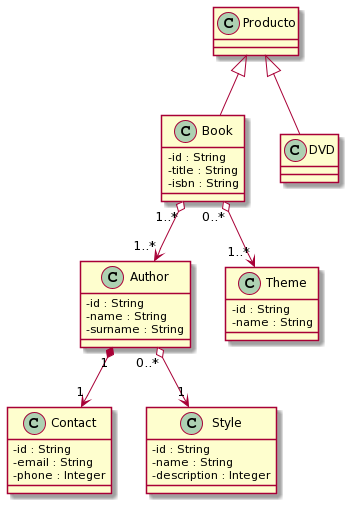
\includegraphics[width=\textwidth]{fig/ejercicioBiblioteca}}

Una posible solución. Notar cómo se representan las dos jeraquías.}
% Pincha en el siguiente enlace
% http://www.plantuml.com/
\end{column}
\end{columns}
\end{frame}
% . . . . . . . . . . . . . . . . . . . . . . . . . . . . . . . . . . . . . . . . . . . . . . . . . . . . . . 
% . . . . . . . . . . . . . . . . . . . . . . . . . . . . . . . . . . . . . . . . . . . . . . . . . . . . . . 
%@startuml
%skinparam classAttributeIconSize 0
%
%
%class Producto{}
%
%class Book {
% - id : String
% - title : String
% - isbn : String
%}
%
%class DVD{}
%
%class Author {
% - id : String
% - name : String
% - surname : String
%}
%
%class Theme {
% - id : String
% - name : String
%}
%
%class Contact {
% - id : String
% - email : String
% - phone : Integer
%}
%
%class Style {
% - id : String
% - name : String
% - description : Integer
%}
%
%Book -up-|> Producto
%DVD -up-|> Producto
%
%Book "1..*" o--> "1..*" Author
%Book "0..*" o--> "1..*" Theme
%Author "1" *--> "1" Contact
%Author "0..*" o--> "1" Style
%@enduml







%%%%%%%%%%%%%%%%%%%%%%%%%%%%%%%%%%%%%
%%%%%%%%%%%%%%%%%%%%%%%%%%%%%%%%%%%%%
\begin{frame}{Ejercicio} \small 
\begin{ejercicio}{}
En un sistema de simulación están los \textbf{agentes} (inteligentes) con  métodos que permiten realizar una toma de \textbf{decisiones} (p.e. con una máquina de estados) y aquellos que además tienen un \textbf{cuerpo} físico y que les permite moverse en el escenario.
\end{ejercicio}

\begin{ejercicio}{}

Todo \textbf{cliente} se caracteriza por tener un DNI y una cuenta bancaria, que puede ser de ahorro o de crédito. Si es de ahorro, genera unos intereses; pero si es de crédito permite tener un depósito. Una cuenta bancaria se crea con un saldo inicial.  En toda cuenta se puede depositar y retirar dinero. Un DNI consta de un identificador junto con el nombre, dirección y edad al que pertenece.
\end{ejercicio}



\begin{ejercicio}{}
Toda \textbf{alarma} tiene un \textbf{umbral} de sensibilidad de intrusos. También consta de un \textbf{sensor} al que consulta y que le indica cual es el valor actual de intrusión. En el caso de que se supere el umbral, puede ocurrir lo siguiente.

Si es una alarma \textbf{sonora}, pondrá en marcha un timbre incorporado que se puede activar o desactivas. Pero si es una alarma \textbf{luminosa}, encenderá una luz. En el caso de que sea sonora y luminosa hará las dos cosas.
\end{ejercicio}

\end{frame}
% . . . . . . . . . . . . . . . . . . . . . . . . . . . . . . . . . . . . . . . . . . . . . . . . . . . . . . 
% . . . . . . . . . . . . . . . . . . . . . . . . . . . . . . . . . . . . . . . . . . . . . . . . . . . . . . 





%%%%%%%%%%%%%%%%%%%%%%%%%%%%%%%%%%%%%
%%%%%%%%%%%%%%%%%%%%%%%%%%%%%%%%%%%%%
\begin{frame}{Ejercicio} \small 
\begin{ejercicio}{}
Para el ejercicio anterior de la alarma ?`qué modificaciones tendrías que hacer para que una alarma completa encendiera la luz ante cierto nivel de intrusión, pero que hiciera sonar también el timbre si el nivel fuera aún mayor?
\end{ejercicio}



\begin{ejercicio}{}
Están los relojes (con sus horas, minutos y segundo), que cada. vez que hacen un tictac avanzan un segundo. También están los calendarios (con sus días, meses y años) que avanzan día a día. Y están los relojes con calendarios. ?`Cómo se construyen? ¿cómo avanzan un segundo? ¿cómo avanzan un día?
\end{ejercicio}




%\begin{itemize}
%\item Un \cm{Vehículo} se caracteriza por su \cm{marca}, \cm{precio}.
%\item Se tienen las subclases \cm{Eléctrico} y \cm{Combustible} con los atributos tiempo de carga (en horas) y fecha de compra (en años).
%
%\item Escribe las interfaces Getter/Setter.
%
%\item Las 3 clases tienen el método \cm{calcular(int)}. Para \cm{Vehículo} y \cm{Eléctrico} se interpreta como el precio total para un número de vehículos dado, y para \cm{Combustible} el parámetro se interpreta como la fecha de venta en años, que disminuye en 1/10 con respecto al año anterior.
%
%
%\item Implementa en el método estático \cm{main()} una prueba unitaria.
%
%\item Cuando termines, pregúntate
%\begin{itemize}
%\item Dónde se usa \cm{this}, \cm{this()}, \cm{super} y \cm{super()}. Justifica.
%\item Qué es la \textbf{sobreescritura} y dónde la estás aplicando.
%\item Qué es la \textbf{sobrecarga} y dónde la estás usando.
%\item Qué es el \textbf{polimorfirmo} y dónde está sucediendo.
%\end{itemize}
%\end{itemize}





\end{frame}
% . . . . . . . . . . . . . . . . . . . . . . . . . . . . . . . . . . . . . . . . . . . . . . . . . . . . . . 
% . . . . . . . . . . . . . . . . . . . . . . . . . . . . . . . . . . . . . . . . . . . . . . . . . . . . . . 





\end{document}
%
%\item http://www.it.uc3m.es/java/git-gisc/units/oo-herencia/slides/ProgramacionOrientadaAObjetos.pdf








